\subsection{Results based on Default Environment}

We next evaluate three learning-based approaches on the same default environment setting (intersection map with static obstacles): PPO (on-policy), SAC (off-policy), and MBPO (model-based off-policy). PPO and SAC are trained for up to 1.6M environment steps using 10 parallel environments, while the final MBPO run is trained for \textbf{610k real environment steps}. The random baseline achieves a mean return of \textbf{6.39}, providing a reference point for learned performance.

\paragraph{PPO (On-Policy)}
PPO improves rapidly during early training, reaching a peak mean return of \textbf{137.4} at approximately \textbf{400k steps}. However, this performance is not sustained. After the peak, returns collapse sharply, dropping close to zero by 800k steps and only partially recovering to $\sim$18 by the end of training. The variability during the peak phase is also high (interquartile range 8--218), indicating inconsistent behavior across evaluation episodes.

\paragraph{SAC (Off-Policy)}
In contrast, SAC exhibits stable and monotonic improvement. After an initial exploration phase, performance steadily increases, reaching \textbf{490.5} at \textbf{1.59M steps}. By approximately 820k steps, all evaluation episodes exceed a return of 50, and performance remains stable thereafter (\textbf{416.7} at the end of training). The interquartile range is significantly narrower than PPO's, indicating consistent policy behavior. SAC's stability can be attributed to its off-policy nature, where the replay buffer retains diverse transitions and prevents collapse even when the current policy degrades. It also achieved a higher and near 100\% success rate.

\paragraph{MBPO (Model-Based Off-Policy)}
The final MBPO run shows faster early improvement than a random policy, but it does not achieve stable task completion. As shown in Figure~\ref{fig:learning_curves_with_mbpo}, MBPO reaches its best mean return of \textbf{110.6} at \textbf{210k real environment steps}, with an interquartile range of \textbf{80.3--142.6}. However, this gain is not sustained. After the peak, the curve oscillates sharply and then collapses, including a severe drop to \textbf{-183.8} at \textbf{390k steps}. The final checkpoint at \textbf{610k steps} ends at \textbf{-4.0} mean return, with \textbf{0\% success rate} and a mean episode length of \textbf{1000}, indicating that the learned policy frequently falls back to horizon-limited, non-terminating behavior.

This pattern suggests that the learned dynamics model helps the agent discover short periods of useful progress-seeking behavior, but that behavior is not robust enough to yield reliable goal reaching. In our setting, MBPO appears to suffer from the same instability seen in PPO, although for a different reason: instead of on-policy collapse, the model-based rollouts do not provide a sufficiently accurate or sufficiently informative signal to consistently learn the final approach to the goal. As a result, MBPO improves over the random baseline early on, but remains substantially less stable and less effective than SAC.

\begin{figure}[t]
    \centering
    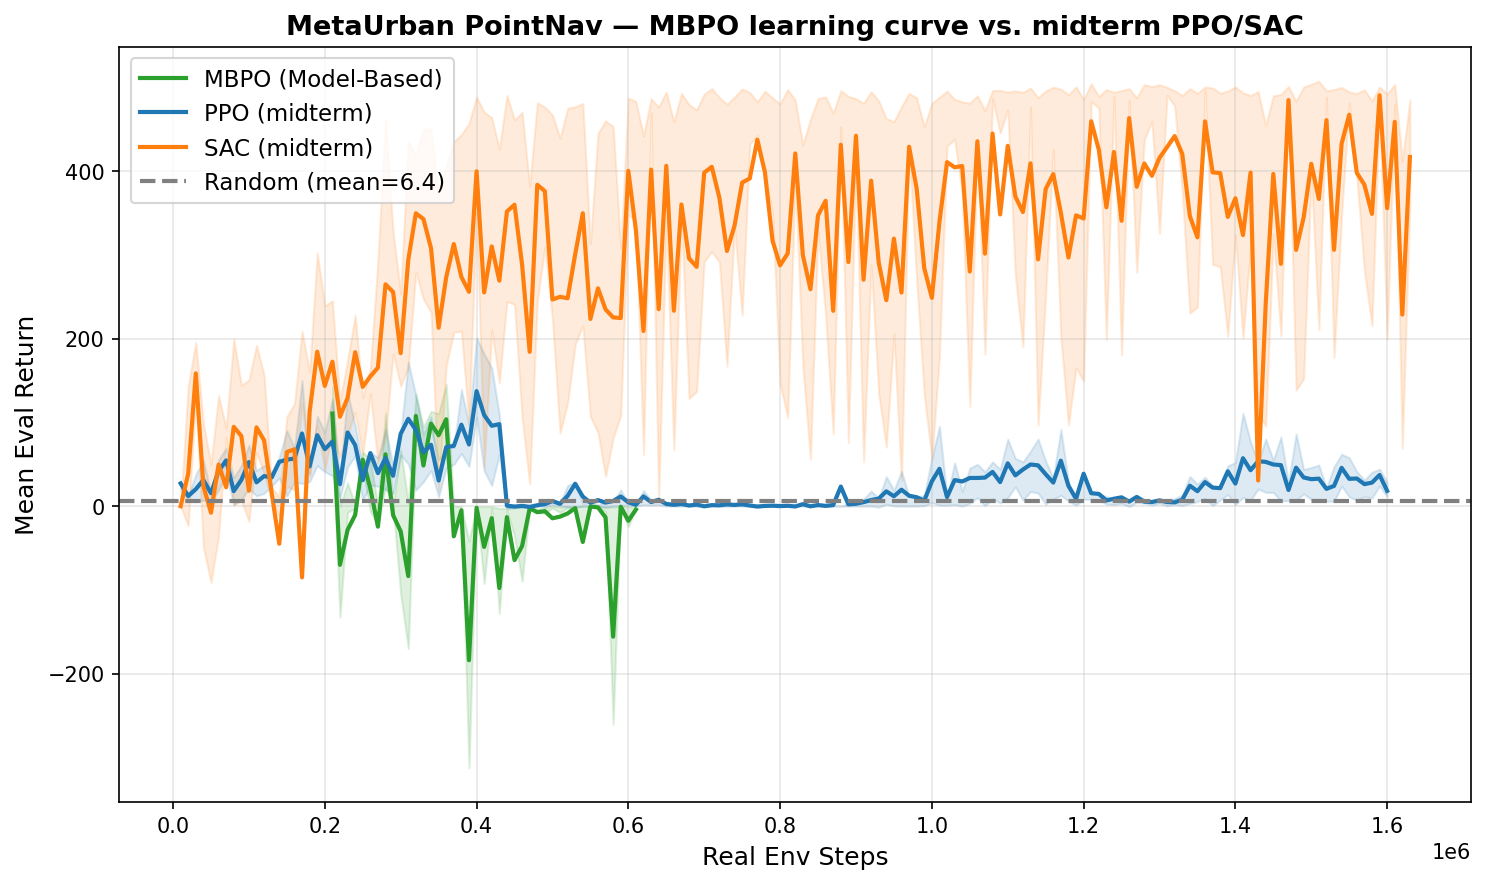
\includegraphics[width=\linewidth]{img/learning_curves_with_mbpo.png}
    \caption{Learning curves for PPO, SAC, and MBPO. The dashed gray line indicates the random baseline. Shaded regions show the 25th--75th percentile across evaluation episodes. MBPO improves early but is markedly less stable than SAC and ultimately collapses.}
    \label{fig:learning_curves_with_mbpo}
\end{figure}

\begin{figure}[h]
    \centering
    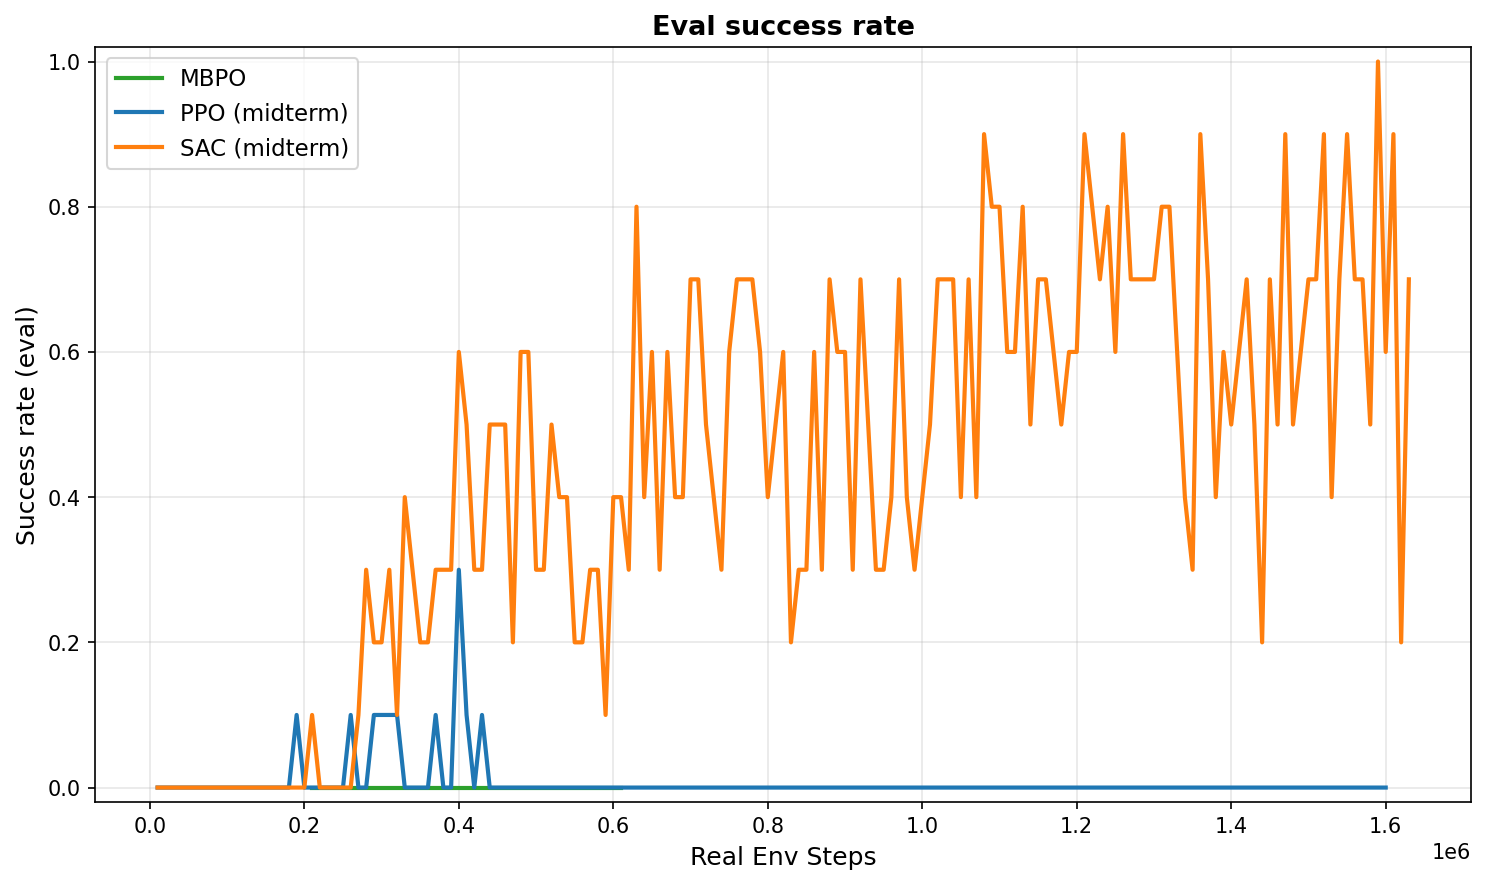
\includegraphics[width=\linewidth]{img/success_rates_with_mbpo.png}
    \caption{Evaluation success rate versus training steps for PPO, SAC, and MBPO. PPO spikes early and then collapses, SAC improves steadily with strong late performance, and MBPO remains at 0\% throughout the final run.}
    \label{fig:success_rates_with_mbpo}
\end{figure}

Overall, SAC provides the strongest and most reliable performance on the default environment. PPO can briefly achieve moderate performance but is unstable, while MBPO improves early yet fails to translate model-based exploration into consistent task success.

The video of PPO, SAC, and MBPO can be found at \href{https://howardhan99.github.io/metaurban/}{https://howardhan99.github.io/metaurban/}.
